%*********************************************************************%
%                                                                     %
%              Introduction section                                   %
%                                                                     %
%*********************************************************************%

\chapter{Elements in Modeling 3-D Stellar Convection and Dynamo Action} %Models of 3-D MHD Convection and Dynamo Action
\label{chapter:ASH}
\label{sec:ASH}

To study the coupling between rotation, magnetism and the
large-scale flows achieved in stellar convection zones, we must
employ a global model which 
simultaneously captures the spherical shell geometry and admits the
possibility of zonal jets and large eddy vortices, and of convective plumes
that may span the depth of the convection zone.  The solar convection
zone is intensely turbulent and microscopic values of viscosity and
magnetic and thermal diffusivities in the Sun are estimated to be very
small.  Numerical simulations cannot hope to resolve all scales of
motion present in real stellar convection and must instead strike a
compromise between resolving dynamics on small scales and capturing
the connectivity and geometry of the global scales. Here we focus on
the latter by studying a full spherical shell of convection.

\section{Anelastic MHD Formulation}
Our tool for exploring MHD stellar convection is the anelastic spherical
harmonic (ASH) code, which is described 
%briefly in \cite{Brown_et_al_2008} and in more 
in detail in \cite{Clune_et_al_1999}.  The implementation of magnetism
is discussed in \cite{Brun_et_al_2004}.   
ASH solves the 3-D MHD anelastic equations of motion in a
rotating spherical shell using the pseudo-spectral method and runs
efficiently on massively parallel architectures. 
We use the anelastic approximation to capture the effects of density
stratification without having to resolve sound waves which have short
periods (about 5 minutes) relative to the dynamical time scales of the
global scale convection (weeks to months) or possible cycles of
stellar activity (years to decades).  This criteria effectively filters
out the fast magneto-acoustic modes while retaining the slow modes and
Alfv\'en waves.
Under the anelastic approximation the thermodynamic fluctuating
variables are linearized about their spherically symmetric and
evolving mean state, with radially varying density $\bar{\rho}$, pressure $\bar{P}$,
temperature $\bar{T}$ and specific entropy $\bar{S}$.  The fluctuations
about this mean state are denoted as $\rho$, $P$, $T$ and $S$.  
In the reference frame of the star, rotating at average rotation rate $\Omega_0$, 
the resulting MHD equations are:
%
\begin{equation}
  \label{eq:div mass flux}
  \vec{\del} \cdot(\avg{\rho}\vec{v}) = 0\thinspace,
\end{equation}\\[-15mm]
%
\begin{equation}
  \label{eq:div B}
  \vec{\del} \cdot\vec{B} = 0\thinspace,
\end{equation}\\[-10mm]
%
\begin{equation}
  \label{eq:momentum}
  \begin{array}{c}
  \displaystyle \avg{\rho}\left[ \frac{\partial\vec{v}}{\partial t} +
    (\vec{v} \cdot \vec{\del})\vec{v} +
    2 \vec{\Omega}_0 \cross \vec{v} \right] 
  =  \qquad\qquad\qquad\qquad\\[3mm]
  \displaystyle
  \qquad\qquad\qquad\qquad  -\vec{\del} (\avg{P} + P) + (\avg{\rho} + \rho) \vec{g}
                +\frac{1}{4 \pi} \left(\vec{\del} \cross \vec{B} \right) \cross \vec{B} 
                -\vec{\del} \cdot \scrD ,
  \end{array}
\end{equation}\\[-5mm]
%
\begin{equation}
  \label{eq:induction}
  \frac{\partial\vec{B}}{\partial t} = 
       \vec{\del} \cross (\vec{v} \cross \vec{B}) - \vec{\del} \cross (\eta \vec{\del} \cross \vec{B}), 
\end{equation}\\[-5mm]
%
\begin{equation}
  \label{eq:entropy}
  \begin{array}{c}
  \displaystyle 
  \avg{\rho}\avg{T}
  \left[\frac{\partial S}{\partial t} + \vec{v} \cdot \vec{\del}(\avg{S}+S)\right]  = \qquad\qquad\qquad\qquad \\[3mm]
  \displaystyle 
  \qquad\qquad\qquad\qquad\qquad \vec{\del} \cdot \left[ \kappa_r \avg{\rho} c_p \vec{\del}(\avg{T}+T) 
                    +\kappa_0 \avg{\rho} \avg{T} \vec{\del} \avg{S}
		    +\kappa \avg{\rho} \avg{T} \vec{\del} S \right] \\[3mm]
  \displaystyle 
  \qquad\qquad\qquad + \frac{4 \pi \eta}{c^2} \vec{j}^2 
  + 2 \avg{\rho}\nu \left[e_{ij}e_{ij} - \frac{1}{3}(\vec{\del} \cdot \vec{v})^2\right],
  \end{array}
\end{equation}\\[-5mm]
where $\vec{v} = (v_r, v_\theta, v_\phi)$ is the local velocity
in the stellar reference frame,
$\vec{B}=(B_r, B_\theta, B_\phi)$ is the magnetic field, $\vec{j}$ is
the vector current density, 
$\vec{g}$ is the gravitational acceleration, 
$c_p$ is the specific heat at constant pressure, 
$\kappa_r$ is the radiative diffusivity and $\scrD$ is the viscous
stress tensor, given by
\begin{equation}
  \scrD_{ij} = -2 \avg{\rho} \nu \left[e_{ij} 
    - \frac{1}{3}(\vec{\del} \cdot \vec{v})\delta_{ij} \right],
\end{equation}
where $e_{ij}$ is the strain rate tensor.  Here $\nu$,
$\kappa$ and $\eta$ are the diffusivities for vorticity,
entropy and magnetic field.  We assume an ideal gas law
\begin{equation}
  \avg{P} = \scrR \avg{\rho} \avg{T},
\end{equation}
where $\scrR$ is the gas constant, and close this
set of equations using the linearized relations for the thermodynamic
fluctuations of
\begin{equation}
  \frac{\rho}{\avg{\rho}} = \frac{P}{\avg{P}} - \frac{T}{\avg{T}}
    =  \frac{P}{\gamma \avg{P}} - \frac{S}{c_p}.
\end{equation}
The mean state thermodynamic variables that vary with radius are
evolved with the fluctuations, thus allowing the convection to modify
the entropy gradients which drive it. 

The mass flux and the magnetic field are represented with a
toroidal-poloidal decomposition as
\begin{eqnarray}
  \avg{\rho}\vec{v} =& \vec{\del}\cross\vec{\del}\cross(W \hat{r}) + \vec{\del}\cross(Z\hat{r}), \\
            \vec{B} =& \vec{\del}\cross\vec{\del}\cross(\beta \hat{r}) + \vec{\del}\cross(\zeta\hat{r}),
\end{eqnarray}
with streamfunctions $W$ and $Z$ and magnetic potentials $\beta$ and $\zeta$.
This approach ensures that both quantities remain divergence-free to
machine precision throughout the simulation.  The velocity, magnetic
and thermodynamic variables are all expanded in spherical harmonics
for their horizontal structure and in Chebyshev polynomials for their
radial structure.  The solution is time evolved with a second-order
Adams-Bashforth/Crank-Nicolson technique.

ASH is a large-eddy simulation (LES) code, with subgrid-scale (SGS)
treatments for scales of motion which fall below the spatial resolution in our
simulations.  We treat these scales with effective eddy diffusivities,
$\nu$, $\kappa$ and $\eta$, which represent the transport of momentum,
entropy and magnetic field by unresolved motions in the simulations. 
In these simulations $\nu$, $\kappa$ and $\eta$ are
taken for simplicity as functions of radius alone and are proportional
to $\bar{\rho}^{-1/2}$.   
This adopted SGS variation, as in \cite{Brun_et_al_2004},
\cite{Browning_et_al_2006} and \cite{Ballot_et_al_2007} 
yields lower diffusivities near the bottom of the layer and thus
higher Reynolds numbers. In their stellar structure, our simulations here
are similar to case~AB as reported in \cite{Brun&Toomre_2002} though with a
different SGS functional form (there $\nu, \kappa \propto \bar{\rho}^{-1}$),
and here we shall consider the effects of faster $\Omega_0$ (there
$\Omega_0 = \Omega_\odot)$.  Acting on the mean entropy gradient is
the eddy thermal diffusion $\kappa_0$ which is treated separately and
occupies a narrow region in the upper convection zone.  Its purpose is
to transport entropy through the outer surface where radial convective
motions vanish.  

Our simulations are still separated
by many orders of magnitude from the intensely turbulent conditions
present within the solar convection zone.  They are
likely to capture many aspects of the dynamics of solar convection, and
we are encouraged by the success that similar simulations 
\citep[e.g.,][]{Miesch_et_al_2000,Brun&Toomre_2002,Miesch_et_al_2006,Miesch_et_al_2008}
have had in beginning to match the detailed observational constraints for
differential rotation within the solar convection zone provided by
helioseismology \citep[c.f.\ ][]{Thompson_et_al_2003}.


\section{Boundary Conditions and Their Impacts}


In this thesis we will explore how patterns of convection and
dynamo-generated magnetism change in more rapidly rotating suns.  In
models of the solar dynamo, the magnetic fields observed at the
surface are thought to be in the convection zone, with the tachocline
of penetration and shear at the base of the convection zone possibly
allowing field to be stored and organized on global-scales.  The
tachocline is a complex internal boundary layer.  Below the tachocline
lies the radiative zone, a region of stable stratification.  Above it
is the intensely turbulent and highly magnetized convection zone.
Plunging downflows originating there splash into the tachocline,
carrying magnetic field downwards and likely driving gravity waves and
large-scale circulations.  In the Sun, the origin and maintenance of
the tachocline remains unclear, but it seems likely that slow
meridional circulations in that layer are crucial to its long term
evolution.  These flows likely have turnover times of millions of
years while the fast downflows in the convection zone evolve on
timescales of a few days.

In nearly all of the simulations contained in this thesis, we will
explore dynamics within the convection zone only.  
Simulations which include model tachoclines are now being conducted in
ASH, with the first simulations of the solar dynamo coupled to a
tachocline reported on in \cite{Browning_et_al_2006}.  Explorations
that include a tachocline will be extended to the rapidly rotating
suns in the future, and preliminary results for such a system will be
shown in Chapter~\ref{chapter:the promise of the future}.  However,
the majority of our simulations here consist of spherical shells of 
convectively unstable fluid which capture the bulk of the solar
convection zone in radius.  We adopt boundary conditions appropriate
to this region, and for now we neglect the region of penetration, shear
and stable stratification at the base of the convection zone.
 
One area of focus in this thesis is the differential rotation which is
naturally established within a shell of fluid that experiences no
external torques.  In these systems, convection and magnetism built by
dynamo action act to redistribute angular momentum within the
convection zone and establish gradients of angular velocity in both
radius and latitude.  Our velocity boundary conditions that are
implemented in ASH are fairly
straight forward and are chosen to eliminate external torques.
The velocity boundary conditions imposed at the top and
bottom of the convectively unstable shell are:
\begin{enumerate}
  \newcounter{BC counter} 
  \item Impenetrable top and bottom: $v_r = 0\thinspace,$
  \item Stress-free top and bottom:
    \begin{equation}
       (\partial/\partial r)(v_\theta/r) =
      (\partial/\partial r)(v_\phi/r) = 0\thinspace, 
    \end{equation}
\end{enumerate}

  In recent solar simulations \citep{Miesch_et_al_2006,
Miesch_et_al_2008} a latitudinal gradient of entropy has been
imposed to mimic the balance likely achieved within the sub-adiabatic
tachocline. This modified boundary condition (with
$S|_\mathrm{r=r_{bot}} = F(\theta)$ constant in time) slightly
modifies the thermal wind balance achieved throughout the convection
zone and can modify the profiles of differential rotation.  The
overall angular velocity contrast in latitude remains similar.  
\cite{Ballot_et_al_2007} explored the consequences of such a boundary
condition in one of their young, rapidly rotating suns with deep
convection zones and found that the results were similar to those of
\cite{Miesch_et_al_2006}. 
In these simulations of rapidly rotating suns however, we do not employ such a
treatment.  Instead, a latitudinal contrast in entropy is naturally
established throughout the convection zone and at the bottom boundary
by the convection itself.  We make this choice
because of our uncertainties about the structure of stellar
tachoclines.  In the case of the Sun, bounds can be placed on this
thermal gradient from helioseismic observations of the tachocline.  

In other stars we have no such asteroseismic observations of their tachoclines.
In the more rapidly rotating suns, we thus do not yet know how the
tachoclines scale with rotation rate, magnetic activity or stellar
age.  As such, the possible thermal structure of those tachoclines is
poorly constrained.  With these observational uncertainties in mind we choose
constant flux thermal boundary conditions and allow the convection to establish its own
gradients of entropy in latitude within the convection zone.  The thermal boundary
conditions at the top and bottom of the shell are thus
\begin{enumerate}
    \setcounter{enumi}{2}
   \item Constant entropy gradient at top and bottom: 
    \begin{equation}
        \partial (S+ \bar{S})/\partial r = \mathrm{const}\:.
    \end{equation}
\end{enumerate}


\section{Magnetic Boundary Conditions}
The most natural choice for the magnetic boundary conditions is
somewhat less clear, and thus deserves some detailed discussion.  
Typically in ASH we employ one of three treatments for magnetism
at the boundaries.  Those conditions are: 
\begin{enumerate}
  %Akward and ugly, but works for now
    \setcounter{enumi}{3}
   \item Match to external potential field at top:
    \begin{equation}
      \vec{B} = \vec{\nabla} \Phi  \quad \mathrm{and} \quad \nabla^2 \Phi = 0 {\big|}_{r=r_\mathrm{top}}\thinspace,\nonumber
    \end{equation}
  \item Perfect conductor at bottom:
    \begin{equation}
      E_\theta = E_\phi = 0\nonumber
    \end{equation}
    \begin{equation}
      B_r = (\partial/\partial r)(r B_\theta)=(\partial/\partial r)(r B_\phi)=0\thinspace,
    \end{equation}
   \item Radial field only at the boundary:
    \begin{equation}
      \vec{B} = B_r\thinspace. \nonumber
    \end{equation}
\end{enumerate}

In our later discussions, it will be helpful to understand the impact
of these different boundary conditions on the transport of angular
momentum and energy through the boundary.  We examine those properties
for each boundary condition in turn.

\subsection{Potential Field Boundaries}

A potential field boundary condition is most appropriate when the
region outside the boundary mimics a vacuum or other extremely good insulator.  Under
the potential field approach, no currents can cross the boundary, nor
can currents be supported in the external volume.  Magnetic fields can
however extend out of the simulation, in a fashion the preserves
$\vec{\nabla}\cdot \vec{B}=0$.  This boundary condition is most
appropriate near the surface of the star, though it entirely neglects
the dynamics present in the photosphere, as well as the complex
balances achieved in the chromosphere of the star and the likely
force-free corona.  The dynamo simulations in this thesis use this as
their upper boundary condition.

Our boundaries are impenetrable to the fluid motions, and thus the
transport of energy by magnetism is from the Poynting flux.  This
flux is
\begin{equation}
  F_\mathrm{Poynting} = S = \frac{c}{4 \pi} \left(\vec{E} \cross \vec{B}\right) = \frac{c}{4 \pi}\Big(\left(-\vec{v} \cross  \vec{B} + \eta \vec{\nabla} \cross \vec{B}\right) \cross \vec{B}\Big)\thinspace,
\end{equation}
where we have used Ohm's law to replace the electric field.  We are
most interested in the flux of energy entering or leaving the volume,
which is given by the radial flux at the boundary.  This is
\begin{equation}
 S_r =  - \frac{c}{4 \pi} \bigg(B_r \left(\vec{B} \cdot \vec{v}\right) + v_r \left( B^2 \right) +
          \eta \Big(\left[\vec{\nabla} \cross \vec{B}\right] \cross\vec{B} \Big)_r\bigg) \thinspace,
\end{equation}
where we use a vector identity to expand the first term in the
electromotive force.  Our impenetrable boundary conditions ensure that
$v_r = 0$.  Using this, and expanding the diffusion term we obtain
\begin{equation}
 S_r =  - \frac{c}{4 \pi} \bigg(B_r \left(\vec{B} \cdot \vec{v}\right) + 
        \eta \left(
	\left[\vec{\nabla} \cross \vec{B}\right]_\theta B_\phi - 
	\left[\vec{\nabla} \cross \vec{B}\right]_\phi B_\theta 
	\right)\bigg)\thinspace.
\label{eq:radial_poynting_flux}
\end{equation}

With a potential field boundary condition, $\vec{B} = \vec{\nabla}
\Phi$ and $\vec{\nabla} \cross \vec{B}=0$, and thus the diffusive terms
vanish.  There is however radial field that can cross the boundary,
and thus an overall energy flux of
\begin{equation}
   S_r =  - \frac{c}{4 \pi} B_r \left(\vec{B} \cdot \vec{v}\right)\thinspace.
\end{equation}
In these simulations, both the mean and fluctuating magnetic fields
contribute to a Poynting flux through the boundary.  The radial fields
enter only through the $B_r$ factor, as $v_r =0$ at the upper surface.
With stress-free boundary conditions, $v_\theta$ and $v_\phi$ are
non-zero.  The horizontal magnetic fields $B_\theta$ and $B_\phi$ can
also be non-zero, though the azimuthally averaged longitudinal field
is zero.  This can be seen from
\begin{equation}
  \langle B_\phi \rangle = \frac{1}{r \sin\theta}\frac{\partial}{\partial \phi} \langle \Phi \rangle =0\thinspace,
\end{equation} 
where angle brackets denote an average in longitude.  This quantity is
zero because there are no longitudinal gradients in the azimuthally
averaged quantities by definition of the average.

There is clearly a fluctuating Poynting flux through a potential field
boundary.  Indeed, the horizontal fields can contribute to a mean
Poynting flux through their correlation with the horizontal flows, and
the colatitudinal  field $B_\theta$ can contribute on both mean and
fluctuating scales, while the longitudinal field
$B_\phi$ contributes only through correlations between the
fluctuating fields and fluctuating velocities.  This mean flux is
given by
\begin{equation}
   \langle S_r \rangle =  
- \frac{c}{4 \pi} 
   \bigg(
   \langle B_r \rangle \Big(
   \langle B_\theta \rangle \langle v_\theta \rangle + 
   \langle B_\theta' v_\theta' \rangle + 
   \langle B_\phi' v_\phi' \rangle \Big)
   +\langle B_r' B_\theta' v_\theta' \rangle + 
   \langle  B_r' B_\phi' v_\phi' \rangle 
   \bigg)\thinspace,
\end{equation}
with fluctuating fields $\vec{B}' = \vec{B} - \langle
\vec{B} \rangle$ and flows $\vec{v}' = \vec{v} - \langle
\vec{v} \rangle$, with again $\langle \vec{B}' \rangle = \langle \vec{v}'
\rangle = 0$ by definition.  Generally, the total Poynting flux across
a shell is very small, as local regions of inward and outward directed
flux tend to cancel one another when an average is taken across both
the northern and southern hemispheres.

%In addition to the transport of energy, we can ask whether magnetic
%flux is transported through a boundary.  At our spherical boundary, 
%this is given by
%\begin{equation}
%  \vec{\hat{r}} \cross \vec{E}
%\end{equation}
%With potential field boundary conditions, this becomes
%\begin{equation}
%  \vec{\hat{r}} \cross \vec{E} = \hat{r} \cross \left(\vec{v} \cross
%  \vec{B}\right) = 
%\end{equation}
%\textbf{which becomes what exactly?}

The transport of angular momentum 
in the hydrodynamic simulations will be discussed later in detail in \S\ref{sec:angular  momentum}.  
In the dynamo simulations, the magnetic contribution to the radial angular momentum flux through
a boundary is given by
\begin{eqnarray}
  F^{MS}_r &=& - \frac{r \sin \theta}{4 \pi} \langle B_r' B_\phi' \rangle\thinspace, \\[3mm] 
  F^{MT}_r &=& - \frac{r \sin \theta}{4 \pi} \langle B_r\rangle \langle B_\phi \rangle\thinspace,
\end{eqnarray}
with $F^{MS}$ the angular momentum transport from fluctuating Maxwell
stresses and $F^{MT}$ the transport by large-scale magnetic torques \citep{Brun_et_al_2004, Brun_et_al_2005}.
At a potential field boundary, $\langle B_\phi \rangle = 0$, thus $F^{MT}$
vanishes.  In principle there could be a remaining flux from the
fluctuating terms; in practice there is not.  Locally there is a flux,
but when integrated over a full shell $F^{MS}_r$ is near zero.  This
is likely related to the nature of the external potential field.  With
no currents and no external forces, the external region is entirely
connected to the simulation and there is no ability to remove
angular momentum entirely from the coupled system.

\clearpage
\subsection{Perfect Conductor Boundaries}

A perfect conductor boundary condition is more appropriate when the
external volume is filled with a plasma that is very highly
conductive.  This boundary condition prevents magnetic field from
crossing the boundary, though currents can flow through.  This
boundary condition seems most appropriate at the bottom of the
convection zone, and it appears that such a boundary condition is more in keeping with the
internal boundary layer that forms when we capture a mock tachocline
within our simulations (see \S\ref{sec:tachocline}).  The dynamo simulations generally have
perfectly conducting bottom boundaries.

Perfect conductor boundaries have no radial Poynting flux.  To show
this, we recall that the horizontal electric fields $E_\theta$ and
$E_\phi$ vanish at the boundary, as does the radial magnetic field.
Thus the radial Poynting flux is
\begin{equation}
  S_r = \frac{c}{4 \pi} \Big( E_\theta B_\phi - E_\phi B_\theta \Big) = 0\thinspace.
\end{equation}
We can see how this feeds into our magnetic boundary conditions by
examining equation~(\ref{eq:radial_poynting_flux}).  At a perfect
conducting boundary, that equation becomes
\begin{eqnarray}
 S_r &=&  -  \frac{c}{4 \pi} B_r \left(\vec{B} \cdot \vec{v}\right) +
        \frac{c}{4 \pi} \frac{\eta}{r} \left(
	\left[\frac{1}{\sin \theta} \frac{\partial}{\partial \phi} B_r - 
	      \frac{\partial}{\partial r}(r B_\phi)\right] B_\phi - 
	\left[\frac{\partial}{\partial r}(r B_\theta) - 
	      \frac{\partial}{\partial \theta} B_r \right] B_\theta 
	\right) \nonumber \\
	&=& - ~0 +
        \frac{c}{4 \pi} \frac{\eta}{r} \left(
	\left[ ~0 - \frac{\partial}{\partial r}(r B_\phi)\right] B_\phi - 
	\left[ \frac{\partial}{\partial r}(r B_\theta) - 0~\right] B_\theta 
	\right) = 0\thinspace,
\end{eqnarray}
and thus our requirement that 
$\partial/\partial r(r B_\theta)=\partial/\partial r(r B_\phi)=0$ at a perfect conductor. 

Perfect conducting boundaries also do not support a radial flux
of angular momentum.  This is guaranteed by the radial field vanishing
at the boundary, which causes both $F^{MS}_r$ and $F^{MT}_r$ to vanish
as well.


\clearpage
\subsection{Radial Field Boundaries}
The last boundary condition, that of a radial field only, is not used
in these dynamo simulations, but has often been important in
magnetoconvection studies where an external field is imposed.  This boundary condition is
numerically simple to implement and corresponds to a system where the
external volume is a region of high magnetic permeability
\citep[e.g.,][pg.~194]{Jackson_1999}.

Radial field boundaries have no Poynting flux.  The
impenetrable condition for velocities $(v_r = 0)$ eliminates the
contribution from $B_r v_r$, and the lack of horizontal magnetic
fields eliminates the radial component of $\left(\vec{\nabla} \cross \vec{B} \right)\cross \vec{B}$.
Likewise, there is no angular momentum flux across this type of
boundary.  This results again from $\langle B_\phi \rangle =0$ and
$B_\phi'=0$ at the boundary.


\subsection{Magnetic Boundary Conditions and Effects on CFL Limits}

The properties of our three possible boundary conditions are
summarized in Table~\ref{table:magnetic boundary conditions}.  
To summarize, the perfectly conducting and radial field only boundary
conditions do not permit a flux of energy or angular momentum across
the boundary and thus in or out of the system.  Potential field
boundary conditions do permit a 
flux of energy and angular momentum, though the azimuthally-averaged
magnetic fields do not contribute to the transport of angular
momentum through the boundary.  Generally, we find that the total flux
of energy or angular momentum through a potential field boundary is
small, as the contributions from the northern and southern hemispheres
largely cancel each other.  Horizontal magnetic fields are permitted
near potential field boundaries and perfectly conducting boundaries,
but are not permitted at a radial field only boundary.  Likewise,
radial magnetic fields can thread through the potential field
boundaries and radial field only boundaries, but are not present at a
perfectly conducting boundary.

\clearpage

\begin{deluxetable}{rcccc}
   \tabletypesize{\footnotesize}
    \tablecolumns{5}
    \tablewidth{0pt}  % `natural' size 
    \tablecaption{Properties of Magnetic Boundary Conditions
    \label{table:magnetic boundary conditions}}
    \tablehead{\colhead{~}  &  
      \colhead{Energy} &
      \multicolumn{2}{c}{Angular Momentum} &
      \colhead{Radial Alfv\'en CFL limited} \\[3mm]
     \multicolumn{1}{c}{Type} &
     \colhead{$S_r$} &
     \colhead{$F^{MS}_r$} &  
     \colhead{$F^{MT}_r$} &
     \colhead{$v_a = \frac{B_r}{\sqrt{4\pi\bar{\rho}}}$}
   }
   \startdata
     Potential Field & 
                     $-\frac{c}{4 \pi} B_r (\vec{B} \cdot \vec{v})$ & 
                     $- \frac{r \sin \theta}{4 \pi} \langle B_r' B_\phi' \rangle $ &
                     %\frac{1}{r\sin\theta}\frac{\partial}{\partial r}\Phi'\frac{\partial}{\partial \phi}\Phi' \rangle $ & 
                     0 &
		     yes \\[3mm]
     Perfect Conductor &
                     0 &
		     0 &
		     0 &
		     no \\[3mm]
     Radial Field &
                     0 &
		     0 &
		     0 &
		     yes \\[3mm]
    \enddata
     \tablecomments{Boundary conditions affect the flux of energy and
      angular momentum in and out of the system.  With some boundary
      choices the simulation may be CFL limited by Alfv\'en waves
      near the boundary.}
%\end{deluxetable*}
\end{deluxetable}

The choice of magnetic boundary conditions can also have direct effect on
the typical timesteps achieved by a simulation.  Our simulations will
become numerically unstable and diverge if we exceed the
Courant-Friedrichs-Lewy (CFL) criteria by taking timesteps which are
too large.  Thus our our timesteps must be shorter than the 
the fastest flow of information between individual grid points.
In dynamo simulations, this becomes an issue with boundary conditions
that permit a radial magnetic field.  Here, Alfv\'en waves traveling
radially encounter the fine grid-spacing inherent to our
Chebyshev expansion.  The CFL timestep limit in the dynamo modeling is
dominated by these relatively rapid waves and becomes
\begin{equation}
  \tau = \alpha_0 \thinspace \tau_{\mathrm{CFL}, \vec{B}}
       = \alpha_0 \left(\frac{v_{A,r}}{\Delta r}\right) 
       = \alpha_0 \left(\frac{B_r}{\sqrt{4 \pi \bar{\rho}}}\frac{1}{\Delta r}\right)\thinspace,
\end{equation}
with $\alpha_0$ a safety factor which is slightly less than unity.

%\clearpage
The limitation arises because we are able in these dynamo
simulations to admit waves which propagate through the narrow grid near
the boundaries.  In contrast, our hydrodynamic simulations of stellar
convection zones do not encounter a similar limitation, as $v_r$
smoothly tends to zero as the boundary is approached, and typically
decreases sufficiently quickly that the narrow grid spacing is not
felt.  Hydrodynamic simulations that include penetration into a stable
layer may of course encounter similar limitations when stacked
Chebyshev domains are used to resolve the internal interface and where
the radial motions are non-zero. In our dynamo simulations,
the Alfv\'en wave CFL timestep, set by waves at the upper potential
field boundary, can be one or two orders of magnitude more stringent
than the limits set by either the convection or the Alfv\'en waves
propagating in the rest of the domain.  In a practical sense, this
stringent CFL limit increases the computational cost of dynamo
simulations with radial field or potential field boundaries by well
over an order of magnitude compared to comparable hydrodynamic cases
or dynamo cases with perfect conducting boundaries at top and bottom.


%\clearpage
\section{Approach to Hydrodynamic Simulations}

%%%%%%%%%%%%%%%%%%%%%%%%%%%%%%%%%%%%%%%%%%%%%%%%%%%%%%%%%%%%%%%%%%%%%

%\begin{deluxetable*}{ccccccccccc}
\begin{deluxetable}{ccccccccccc}
\rotatedeluxetable
   \tabletypesize{\footnotesize}
    \tablecolumns{11}
    \tablewidth{0pt}  % `natural' size 
    \tablecaption{Parameters for Primary Hydrodynamic Simulations
    \label{table:sim parameters}}
    \tablehead{\colhead{Case}  &  
     \colhead{ $N_r, N_\theta, N_\phi$} &
     \colhead{Ra} &  
     \colhead{Ta} &  
     \colhead{Re} &  
     \colhead{$\mathrm{Re}'$} &  
     \colhead{Ro} &
     \colhead{Roc} &   
     \colhead{$\nu$} &  
     \colhead{$\kappa$} &  
     \colhead{$\Omega_0/\Omega_\sol$}
   }
   \startdata
                 G1 & $96 \times 256 \times 512$ & 
		      $ 3.22 \times 10^{4} $ & $ 3.14 \times 10^{5} $ &
		      $\phn\phn  84$ & $ \phn 63$ & $  0.92$ & $  0.61$ & $  2.75 $ & 
		      $ 11.0  $ & $ 1$ \\
                 G2 & $96 \times 256 \times 512$ & 
		      $ 1.75\times 10^{5} $ & $ 3.21\times 10^{6} $ & 
		      $\phn 205$ & $ \phn 85$ & $  0.55$ & $  0.45$ & $  1.72 $ &
		      $  6.87  $ & $ 2$ \\
                 G3 & $96 \times 256 \times 512$ & 
		      $ 4.22\times 10^{5} $ & $ 1.22\times 10^{7} $ & 
		      $\phn 326$ & $ 103$ & $  0.41$ & $  0.36$ & $  1.32  $ & 
		      $  5.28  $ & $ 3$ \\
                 G4 & $96 \times 256 \times 512$ & 
		      $ 7.89\times 10^{5} $ & $ 3.18\times 10^{7} $ & 
		      $\phn 433 $ & $ 119$ & $  0.33$ & $  0.31$ & $  1.09  $ & 
		      $  4.36  $ & $ 4$ \\
                 G5 & $96 \times 256 \times 512$ & 
		      $ 1.29\times 10^{6} $ & $ 6.70\times 10^{7} $ & 
		      $\phn 543$ & $ 133$ & $  0.28$ & $  0.27$ & $  0.94  $ & 
		      $ 3.76  $ & $ 5$ \\
                 G7 & $192 \times 512 \times 1024$ & 
		      $ 2.63\times 10^{6} $ & $ 2.06\times 10^{8} $ & 
		      $\phn 763$ & $ 154$ & $  0.22$ & $  0.22$ & $  0.75  $ & 
		      $  3.01  $ & $ 7$ \\
                G10 & $192 \times 512 \times 1024$ &
		      $ 5.58\times 10^{6} $ & $ 6.74\times 10^{8} $ & 
		      $1051$ & $ 188$ & $  0.17$ & $  0.18$ & $  0.59  $ & 
		      $  2.37  $ & $10$ \\[0.25cm]
                %
                G3a & $96  \times 256 \times 512$ &
		      $ 7.83\times 10^{5} $ & $ 2.41\times 10^{7} $ & 
		      $\phn 528$ & $ 158$ & $  0.50$ & $  0.34$ & $  0.94  $ & 
		      $  3.76  $ & $ 3$ \\
                G3b & $192 \times 256 \times 512 \phn$ &
		      $ 2.26\times 10^{6} $ & $ 8.02\times 10^{7} $ & 
		      $1121$ & $ 324$ & $  0.70$ & $  0.32$ & $  0.52  $ & 
		      $  2.06  $ & $ 3$ \\
                G5b & $192 \times 512 \times 1024$ & 
		      $ 4.03\times 10^{6} $ & $ 2.23\times 10^{8} $ & 
		      $1347$ & $ 274$ & $  0.41$ & $  0.26$ & $  0.52  $ & 
		      $  2.06  $ & $ 5$ \\[0.1cm]
     \enddata
     \tablecomments{All simulations have inner radius 
	$r_\mathrm{bot} = 5.0 \times 10^{10}$cm and outer radius of 
        $r_\mathrm{top} = 6.72 \times 10^{10}$cm, with 
	$L = (r_\mathrm{top}-r_\mathrm{bot}) = 1.72 \times 10^{10}$cm
	the thickness of the spherical shell.
	%
	Evaluated at mid-depth are the
	%
	Rayleigh number $\mathrm{Ra} = (-\partial \rho / \partial S)
	(\mathrm{d}\bar{S}/\mathrm{d}r) g L^4/\rho \nu \kappa$, 
	the Taylor number $\mathrm{Ta} = 4 \Omega_0^2 L^4 / \nu^2$, 
	the rms Reynolds number $\mathrm{Re}  = v_\mathrm{rms} L /\nu$ and
	fluctuating Reynolds number $\mathrm{Re}' = v_\mathrm{rms}' L /\nu$,  
	the Rossby number $\mathrm{Ro} = \omega / 2 \Omega_0$ ,
	and the convective Rossby number 
	$\mathrm{Roc} = (\mathrm{Ra}/\mathrm{Ta} \mathrm{Pr})^{1/2}$.
	Here the fluctuating velocity $v'$ has the differential rotation removed: $v' = v -
	\langle v \rangle$, with angle brackets denoting an average in longitude.
	The Prandtl number $\mathrm{Pr} = \nu / \kappa$ is 0.25 for all simulations.  
	The viscous and thermal diffusivity, $\nu$ and $\kappa$, are
	quoted at mid-depth (in units of $10^{12}~\mathrm{cm}^2\mathrm{s}^{-1}$).
        The rotation rate of each reference frame $\Omega_0$ is in multiples
        of $\Omega_\sol=2.6 \times 10^{-6}~\mathrm{rad}~\mathrm{s}^{-1}$ or $414$ nHz.  The~viscous
	time scale at mid-depth $\tau_\nu = L^2/\nu$ is $1250$~days for case G1 and
	is $3640$~days for case G5.  Additional cases considered other
	rotation rates at $1.25, 1.5, 1.75$ and $6~\Omega_\sol$.     
	}
%\end{deluxetable*}
\end{deluxetable}

%%%%%%%%%%%%%%%%%%%%%%%%%%%%%%%%%%%%%%%%%%%%%%%%%%%%%%%%%%%%%%%%%%%%%



%\subsection{Hydrodynamic Studies of Global-Scale Convection in G-type Stars}
Our numerical model is a relatively simple description of the solar
convection zone that captures the essential spherical geometry and
global connectivity of that domain.  Solar values are taken for heat
flux, mass and radius and a perfect gas is assumed.  Near the solar
surface the H and He ionization zones, coupled with radiative losses,
drive intense convective motions on very small scales which appear at
the surface as granulation.  Capturing granulation in a global
simulation would require spherical harmonic degrees of order 4000 and
this is currently too demanding.  We therefore position the top of our
domain slightly below these ionization layers.  In these simulations
our lower boundary is positioned near the base of the
convection zone, thus omitting the stably stratified
radiative interior and the shear layer at the base of the convection
zone known as the tachocline.  We make this choice both because the
nature of tachoclines in rapidly rotating stars is quite uncertain at
present and because simulations that include penetration into a stable
region are quite challenging in terms of computational resources. 

\clearpage
We focus here on the bulk of the convection zone, with our computational
domain extending from $0.72R_{\sol}$ to $0.965R_{\sol}$, thus spanning
172~Mm in radius.  The total density contrast across the shell is
about 25.  The reference or mean state of our thermodynamic variables
is derived from a one-dimensional solar structure model
\citep{Brun_et_al_2002} and is continuously updated with the
spherically symmetric components of the thermodynamic fluctuations as
the simulations proceed.  These values are illustrated in
Figure~\ref{fig:ash_structure} after convection has readjusted the
stratification.

 
%%%%%%%%%%%%%%%%%%%%%%%%%%%%%%%%%%%%%%%%%%%%%%%%%%%%%%%%%%%%%%%%%%%%%
\begin{figure}[htbp]
  \begin{center}
    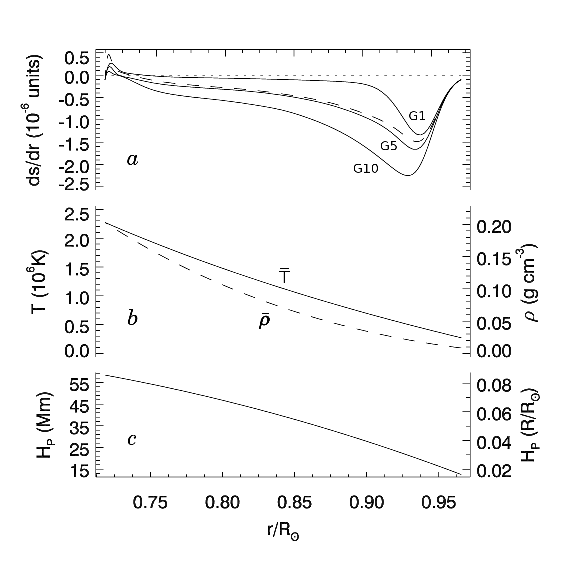
\includegraphics[width=0.75\linewidth]{figs/chapter_2/Figure_1.eps}
  \end{center}
  %\plotone{f1.eps}
  \caption[Radial variation of mean stellar structure in the ASH models]
          {Radial variation of mean stellar structure in the ASH models.  
  $(a)$~Entropy gradient ($\mathrm{d}\bar{S}/\mathrm{d}r$) for cases~G1, G5
  and G10 (as labeled).  At higher rotation rates the entropy gradient
  becomes steeper throughout the convection zone, even for our most
  turbulent cases (case~G5b, long dashes).  $(b)$~Temperature and
  density (latter ranging from 0.203 to 0.008 $\mathrm{g}\thinspace
  \mathrm{cm}^{-3}$ in the region simulated) for case~G1.  
  $(c)$~Pressure scale height $H_P$ (in Mm and fractional solar radii), for
  case~G1, with cases~G2-G10 similar in their mean stratification.
  \label{fig:ash_structure}}
  %\vspace{0.5cm}
\end{figure}
%%%%%%%%%%%%%%%%%%%%%%%%%%%%%%%%%%%%%%%%%%%%%%%%%%%%%%%%%%%%%%%%%%%%%
 


Our hydrodynamic studies here explore a variety of solar-like stars
rotating from $1$ to $10~\Omega_\sol$ (cases~G1-G10).  All cases use
the same initial stellar structure.
%
We seek to explore the general effects of rotation on stellar
convection rather than the evolution of a particular star, which would
require modifications to the stellar structure as the star aged.  In
surveying the effects of more rapid rotation on global-scale
convection, we seek to achieve reasonably high levels of turbulence
in the resulting flows.  Thus our trajectory through the parameter
space of $\Omega_0, \nu,$ and $\kappa$ attempts to maintain strong
nonlinearity without having the increasing $\Omega_0$ serve to laminarize the
convection.
%
As we increase the rotation rate, we simultaneously decrease the
effective eddy diffusivities $\nu$ and $\kappa$ to maintain the
supercriticality of the simulated turbulent convection.  We note that
the critical Rayleigh number for the onset of convection scales with
rotation as $\mathrm{Ra}_c \propto \mathrm{Ta}^{2/3} \propto \Omega_0^{4/3}\nu^{-4/3}$ for Boussinesq
convection \citep[e.g.,][]{Chandrasekhar_1961, Dormy_et_al_2004}.
Lower diffusivities lead to both longer viscous and thermal diffusion
time scales and to flows possessing finer spatial scales.  Achieving
equilibrated states in these systems requires high resolution
simulations carried out over extended periods.  We have taken a middle
ground between attempting to maintain constant supercriticality (which
may require scaling $\nu, \kappa \propto \Omega_0^{-2}$) and keeping
resolution requirements reasonable by scaling our diffusivities as
$\nu, \kappa \propto \Omega_0^{-2/3}$.  All of our cases studied
are highly supercritical, noting that the critical Rayleigh
number for these simulations at $1~\Omega_\odot$ is $\mathrm{Ra}_c
\thinspace \sim \thinspace 1000$ \citep{Gilman&Glatzmaier_1981,
Miesch_thesis}.  We have also maintained a constant Prandtl number
$\mathrm{Pr} = \nu / \kappa = 0.25$ in all of our simulations.  The
parameters of our models are detailed in Table~\ref{table:sim
parameters}.  Our choice of scalings for the eddy diffusivities with
rotation rate may have some influence on the nature of the convective
patterns and mean flows we achieve. To assess some of the sensitivity
the choice of our path through parameter space, we have also sampled a
limited range of more turbulent simulations at a few rotation rates
(cases G3a, G3b and G5b).

Some of our simulations are initialized by perturbing a quiescent
state in solid body rotation.  The growth of convection leads to
velocity correlations that serve to redistribute angular momentum
within the shell, building a differential rotation and meridional
circulation.  We evolve the simulation for long periods compared
variously to convective overturning times, rotation periods or typical
diffusive times.  Other simulations were started from these evolved
states and then run for long intervals after all adjustments have been
made to the frame rotation rate $\Omega_0$ and to the viscous and
thermal diffusivities.  

All of the hydrodynamic simulations discussed in this thesis are at approximately the same
level of maturity in their evolution.  Case~G1 was the progenitor case
at $1~\Omega_\sol$ and was evolved for some 3000 days after branching
away from case~AB from \cite{Brun&Toomre_2002}, which itself has seen
about 10000 days of total simulated life.  Starting with this case,
each subsequent simulation was spun up from the next fastest case
(i.e., G3 was spun up from G2) and evolved for over 4000 days, or many
hundreds of rotation periods.  


%%%%%%%%%%%%%%%%%%%%%%%%%%%%%%%%%%%%%%%%%%%%%%%%%%%%%%%%%%%%%%%%%%%%%
\begin{figure}[htbp]
  \begin{center}
    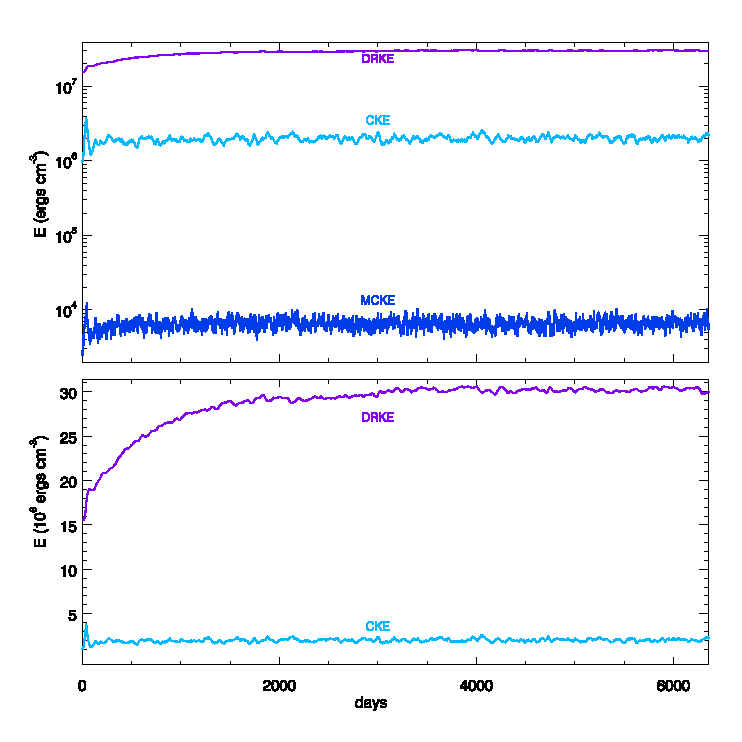
\includegraphics[width=0.85\linewidth]{figs/chapter_2/apj_energy_trace_ab2_turf5.eps}
  \end{center}
  \caption[Evolution of kinetic energies in hydrodynamic case~G5]
	  {Evolution of kinetic energies in hydrodynamic case~G5. $(a)$
	  Volume-averaged kinetic energy densities of differential
	  rotation (DRKE), convection (CKE) and meridional
	  circulations (MCKE) shown in logarithmic plot for the first
	  6500 days of the simulation.  Convective
	  kinetic energies adjust very quickly, but the energy of the
	  mean circulations take longer to equilibrate.  After
	  approximately 4000~days all three energies have reached a
	  stationary state. $(b)$ Linear plot of evolving DRKE and CKE.
  \label{fig:energy_G5}}
  %\vspace{0.5cm}
\end{figure}
%%%%%%%%%%%%%%%%%%%%%%%%%%%%%%%%%%%%%%%%%%%%%%%%%%%%%%%%%%%%%%%%%%%%%

The time evolution of case~G5, which was
started from an evolved state, is shown in
Figure~\ref{fig:energy_G5}.  At day zero the rotation rate $\Omega_0$
and eddy diffusivities $\nu$ and $\kappa$ are set to appropriate
values for case~G5.  The convection responds and equilibrates to these
changes on a timescale of a few
hundred days but the mean flows of differential rotation and
meridional circulation take significantly longer to fully
equilibrate.  As shown in Figure~\ref{fig:energy_G5}$b$ the
differential rotation can take nearly 4000~days to equilibrate.
During this interval the convection and meridional circulations are
redistributing angular momentum and heat, building a latitudinal
contrast of angular velocity and of temperature with hot poles, cool
mid-latitudes and a warm equator (see Chapter~\ref{chapter:convection in G1-G10}). 
After 4000~days the profile of differential rotation remains nearly steady
and we are able to explore the time evolution of the patterns of convection.


After similar intervals of evolution, all cases appear to be
statistically stationary in terms of the angular momentum fluxes and
the kinetic energies.  We believe that the differential rotation
profiles presented are effectively stationary, though there are small
fluctuations as determined from short averages over a few rotation
periods.  Certain cases (including~G5) were evolved for much longer
intervals (over 10000~days and more than 2000 rotation periods) to
explore the long-term behavior of convective patterns in these rapidly
rotating systems.  To test that our results are not unduly subject to
hysteresis in the system, we explored a branch of cases which were
successively spun down from $5~\Omega_\sol$ to $1~\Omega_\sol$.  No
significant hysteresis was found.

We shall discuss the properties of cases G1-G10 in 
Chapters~\ref{chapter:convection in G1-G10} and 
\ref{chapter:active nests of convection}, and there explore the nature
of the convective patterns realized, as well as the
differential rotation and meridional circulation that are achieved for
a range of rotation rates.

\section{Hydrodynamic Progenitors to Dynamo Simulations}

The hydrodynamic progenitors used in our dynamo solutions are slightly
different from the solutions presented as cases G1-G10.
In conducting those hydrodynamic studies, we
learned that at the highest rotation rates the unresolved flux carried
out the top of the domain by $\kappa_0$ was beginning to imprint
deeper into the convection zone.  This occurs because
$\mathrm{d}\bar{S}/\mathrm{d}r$ generally increases in amplitude in
the more rapidly rotating simulations. 

In most of the hydrodynamic
simulations, the $\kappa_0$ diffusion term has the form 
\begin{equation}
  \kappa_0 = \kappa_{0,\mathrm{top}} \left(\frac{\bar{\rho}_\mathrm{top}}{\bar{\rho}}\right)^\alpha + \kappa_{0,\mathrm{C}}
\end{equation}
with $\kappa_{0,\mathrm{top}}$ the diffusivity at the top boundary,
and $\kappa_{0,\mathrm{C}}$ a small constant (of order $10^{10}\thinspace\mathrm{cm}^2\thinspace\mathrm{s}^{-1}$) added to
smooth out potential spikes in $\mathrm{d}\bar{S}/\mathrm{d}r$ near
the bottom of the convection zone, and $\alpha$ controlling the
tapering of the unresolved flux in radius.  
The value of $\kappa_{0,\mathrm{top}}$ is chosen to transport a solar luminosity
through the upper boundary, with
\begin{equation}
  L_u\big|_{r=r_\mathrm{top}} = \left(4\pi r^2 \kappa_0 \avg{\rho} \avg{T} \vec{\del} \avg{S}\right)\big|_{r=r_\mathrm{top}} = L_\odot.
\end{equation}
In all of these rapidly rotating simulations $\kappa_{0,\mathrm{top}} = 2.979 \times
10^{14}$, based on the self-consistently determined profiles of
entropy, temperature and density within ASH.



In cases G1-G10, we chose $\alpha=4$.  Larger values of $\alpha$ lead
to stronger confinement of the unresolved flux to the top of the
convection zone, but also lead to heating within the entropy equation
and modification of the entropy gradients.  Thus, in cases~H3 and H5,
we chose $\alpha=7$ to better confine the unresolved flux in a narrow
upper boundary layer.  As a
result, this flux is largely confined within the upper 10\% of the
convection zone and shows only small variations with rotation rate.

%%%%%%%%%%%%%%%%%%%%%%%%%%%%%%%%%%%%%%%%%%%%%%%%%%%%%%%%%%%%%%%%%%%%%
\begin{figure}[!t]
  \begin{center}
    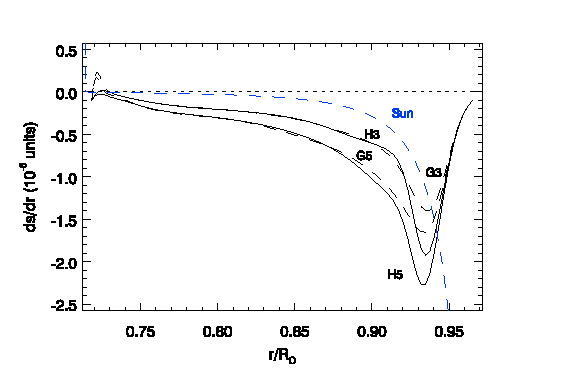
\includegraphics[width=0.75\linewidth]{figs/chapter_2/thesis_dynamo_ASH_structure.eps}
  \end{center}
  %\plotone{f1.eps}
  \caption[Radial structure of dynamo progenitor simulations]
	  {Radial structure of dynamo progenitor simulations.  
	  Shown is the entropy gradient ($\mathrm{d}\bar{S}/\mathrm{d}r$) for
	  dynamo progenitor cases~H3 and H5 (solid lines) 
	  compared with hydrodynamical cases~G3 and G5 (dashed lines).  
	  The entropy gradient in the dynamo progenitor cases is somewhat steeper
	  throughout the convection zone, and the minimum is deeper.
	  This leads to higher Rayleigh numbers in these simulations
	  and stronger driving.  Though the convection is driven more
	  strongly, the temperature, density and pressure profiles are
	  nearly identical to those shown in
	  Figure~\ref{fig:ash_structure}.  Overlain with a blue,
          dashed line is a 1-D solar structure model computed with the
          CESAM code by \cite{Brun_et_al_2002}.
	  \label{fig:ash_dynamo_structure}}
  %\vspace{0.5cm}
\end{figure}
%%%%%%%%%%%%%%%%%%%%%%%%%%%%%%%%%%%%%%%%%%%%%%%%%%%%%%%%%%%%%%%%%%%%%

In these cases the profile of $\mathrm{d}\bar{S}/\mathrm{d}r$ is
somewhat steeper near the top of the convection zone.  This effect is
visible in Figure~\ref{fig:ash_dynamo_structure}, where the stellar
structure of cases~H3 and H5 are compared with that in cases~G3 and
G5.  The profiles of $\mathrm{d}\bar{S}/\mathrm{d}r$ come into good
agreement at depths below $0.87 R_\odot$ for both branches of
simulations, but are deeper for cases H3 and H5 near the top of the
convection zone.  This leads to somewhat stronger driving of the
convection as the Rayleigh numbers are also higher near the top of the
domain.  This partially explains why cases H3 and H5 have higher
Reynolds numbers and higher Rossby numbers (Table~\ref{table:dynamo_sim_parameters})
than cases G3 and G10 (Table~\ref{table:sim parameters}).  The
effects of this are subtle, resulting primarily in slightly stronger
latitudinal gradients of differential rotation and temperature in the
uppermost regions of the shell.  

The entropy gradient from a 1-D, helioseismically-constrained solar
structure model is also shown in Figure~\ref{fig:ash_dynamo_structure}.  
The equilibrated profiles of $\mathrm{d}\bar{S}/\mathrm{d}r$ in ASH
tend to be somewhat steeper than the solar model at depths below
$0.95\: R_\odot$ and significantly shallower in the upper convection
zone.  The large change in $\mathrm{d}\bar{S}/\mathrm{d}r$ between
about $0.93\: R_\odot$ and the surface appears to result from heating
in that layer by our adopted unresolved flux.  New simulations are now
being explored in ASH, with different treatments of the unresolved
flux, and these models appear able to better match the structure
of $\mathrm{d}\bar{S}/\mathrm{d}r$ from the solar model.  Here
however, all of our simulations have $\mathrm{d}\bar{S}/\mathrm{d}r$  
profiles akin to those illustrated in Figure~\ref{fig:ash_dynamo_structure}. 

\clearpage
Convective structures in these hydrodynamic progenitor cases are
similar to those realized in cases~G1-G10, though the patterns tend to
be slightly more complex near the top of the shell.
The patterns of convection for cases~G5 and H5 are shown in
Figure~\ref{fig:five_solar_hydro_cases}.  Shown in global Mollweide
projection are radial velocities at a radius of
$0.95\thinspace R_\odot$ and near the upper boundary. 
These cases were well evolved and possess intricate convective
patterns and solar-like differential rotation profiles, with fast
zonal flow at the equator and slower flows at the poles.
The prominent modulation visible in case~G5
(Fig.~\ref{fig:five_solar_hydro_cases}$a$) is less visible in case~H5.
Here in case~H5 fine-scaled convection has filled in 
the regions between the patches and obscures the modulation. 
These modulated convective states, called
active nests of convection, will be explored in detail in
Chapter~\ref{chapter:active nests of convection} for case~G5 and G10.
Time-longitude maps indicate that these structures are still present
in case~H5 and remain comparable in amplitude to those seen in case~G5.

%%%%%%%%%%%%%%%%%%%%%%%%%%%%%%%%%%%%%%%%%%%%%%%%%%%%%%%%%%%%%%%%%%%%%
\begin{figure}[!p]
  \begin{center}
    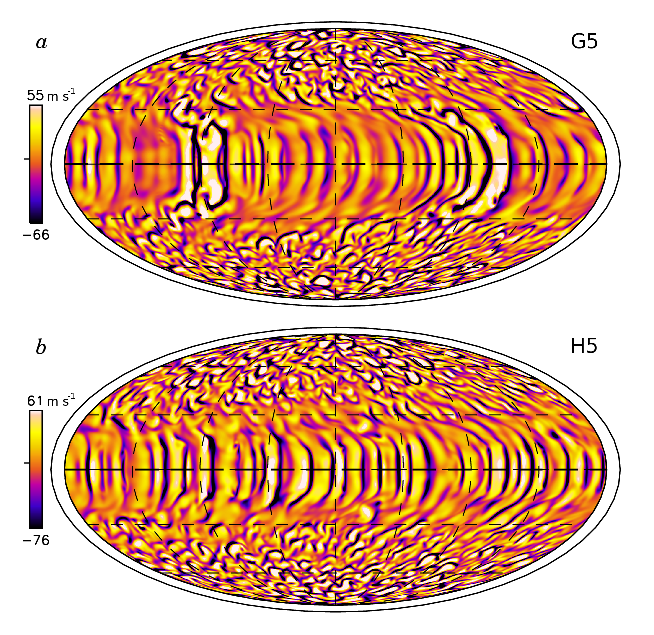
\includegraphics[width=0.8\linewidth]{figs/chapter_2/five_solar_hydro_cases.eps}
  \end{center}
  %\plotone{f1.eps}
  \caption[Patterns of convection in cases~G5 and H5]
	  {Patterns of convection in cases~G5 and H5.  $(a)$ Snapshot
	  of radial velocity $v_r$ in global Mollweide projection for case~G5
	  near the upper boundary ($0.95 \thinspace R_\odot$) with scale
	  indicated.  Downflows are dark and narrow, while upflows are
	  broad and indicated by light tones. A prominent modulation
	  in longitude is visible near the equator.  These active
	  nests of convection persist for thousands of days.
	  $(b)$~Radial velocities in case~H5 at same depth, showing somewhat more vigorous
	  convection.  Here the active nests are obscured by the
	  finer-scale convection but are still visible over long
	  intervals of time.
	  \label{fig:five_solar_hydro_cases}}
  %\vspace{0.5cm}
\end{figure}
%%%%%%%%%%%%%%%%%%%%%%%%%%%%%%%%%%%%%%%%%%%%%%%%%%%%%%%%%%%%%%%%%%%%%




Ultimately, these changes in stratification are modest compared to the
overall structure of the star. As such, the profiles of density,
temperature and pressure are nearly unaffected by the changes in the
entropy gradient.

 
 






\section{Studies of Dynamo Action in Rapidly Rotating Suns}
%\section{Posing the Dynamo Problem}
We have explored a number of dynamo scenarios in our rapidly rotating
suns.  Two solutions, one rotating at three times the current solar
rate ($3\thinspace\Omega_\odot$) and one rotating five times the solar
rate ($5\thinspace\Omega_\odot$), will be the primary
focus of our discussion of dynamo action in Chapters~\ref{chapter:case D3},
\ref{chapter:case D5} and \ref{chapter:dynamo production}.  We begin here by discussing the
basic formulation of the dynamo studies.  The parameter space explored by
our broader family of dynamos will be discussed in turn in
Chapter~\ref{chapter:menagerie of dynamos}. 


%\clearpage
The dynamo simulations were initiated from mature hydrodynamic
progenitor cases which had been evolved for at least 5000 
days at each rotation rate and were well equilibrated.  
Our simulations at three and five times the solar rate
$\Omega_\sol$ lie again on a path where the SGS 
diffusivities $\nu$, $\kappa$ and $\eta$ decrease as
$\Omega_0^{-2/3}$, in order to maintain vigorous convection as rotation
attempts to constrain and quench the motions.  
The fundamental characteristics of our primary dynamo simulations 
and their hydrodynamic progenitors are summarized in
Table~\ref{table:dynamo_sim_parameters}; other cases will be defined
in Chapter~\ref{chapter:menagerie of dynamos}. 

%\begin{deluxetable*}{ccccccccccccc}
\begin{deluxetable}{ccccccccccccc}
\rotatedeluxetable

   \tabletypesize{\footnotesize}
    \tablecolumns{13}
    \tablewidth{0pt}  % `natural' size 
    \tablecaption{Parameters for Primary Dynamo Simulations
    \label{table:dynamo_sim_parameters}}
    \tablehead{\colhead{Case}  &  
      \colhead{$N_r,N_\theta,N_\phi$} &
      \colhead{Ra} &
      \colhead{Ta} &
      \colhead{Re} &
      \colhead{Re$'$} &
      \colhead{Rm} &
      \colhead{Rm$'$} &
      \colhead{Ro} &
      \colhead{Roc} &
      \colhead{$\nu$} &
      \colhead{$\eta$} &
      \colhead{$\Omega_0/\Omega_\sol$}
   }
   \startdata
    D3    & $96 \times 256 \times 512$ & 3.22$ \times 10^{  5}$ &     1.22$ \times 10^{  7}$ & 173 &  105 &   86 &   52 &    0.378 &    0.311 &     1.32 &     2.64 &  3 \\
    D5    & $96 \times 256 \times 512$ & 1.05$ \times 10^{  6}$ &     6.70$ \times 10^{  7}$ & 273 &  133 &  136 &   66 &    0.273 &    0.241 &    0.940 &     1.88 &  5 \\
%
    H3    & $96 \times 256 \times 512$ & 4.10$ \times 10^{  5}$ &     1.22$ \times 10^{  7}$ & 335 &  105 &  --- &  --- &    0.427 &    0.353 &     1.32 &     --- &  3 \\
    H5    & $96 \times 256 \times 512$ & 1.27$ \times 10^{  6}$ &     6.70$ \times 10^{  7}$ & 576 &  141 &  --- &  --- &    0.303 &    0.268 &    0.940 &     --- &  5 \\ 
    \enddata
 \tablecomments{Dynamo simulations at three and five times the solar rotation
    rate are cases D3 and D5, and their hydrodynamic (non-magnetic) companions are H3
    and H5.  
        All simulations have inner radius 
	$r_\mathrm{bot} = 5.0 \times 10^{10}$cm and outer radius of 
        $r_\mathrm{top} = 6.72 \times 10^{10}$cm, with 
	$L = (r_\mathrm{top}-r_\mathrm{bot}) = 1.72 \times 10^{10}$cm
	the thickness of the spherical shell.
	%
	Evaluated at mid-depth are the
	%
	Rayleigh number $\mathrm{Ra} = (-\partial \rho / \partial S)
	(\mathrm{d}\bar{S}/\mathrm{d}r) g L^4/\rho \nu \kappa$, 
	the Taylor number $\mathrm{Ta} = 4 \Omega_0^2 L^4 / \nu^2$, 
	the rms Reynolds number $\mathrm{Re}  = v_\mathrm{rms} L /\nu$ and
	fluctuating Reynolds number $\mathrm{Re}' = v_\mathrm{rms}' L /\nu$,
	the magnetic Reynolds number $\mathrm{Rm} = v_\mathrm{rms} L/\eta$ 
	and fluctuating magnetic Reynolds number 
        $\mathrm{Rm}' = v_\mathrm{rms}' L/\eta$, 
	the Rossby number $\mathrm{Ro} = \omega / 2 \Omega_0$ ,
	and the convective Rossby number 
	$\mathrm{Roc} = (\mathrm{Ra}/\mathrm{Ta} \, \mathrm{Pr})^{1/2}$.
	Here the fluctuating velocity $v'$ has the axisymmetric
        component removed: $v' = v - \langle v \rangle$, 
        with angle brackets denoting an average in longitude.
	For all simulations, the Prandtl number $\mathrm{Pr} = \nu / \kappa$ is 0.25 
	and the magnetic Prandtl number $\mathrm{Pm}=\nu/\eta$ is 0.5.  
	The viscous and magnetic diffusivity, $\nu$ and $\eta$, are
	quoted at mid-depth (in units of $10^{12}~\mathrm{cm}^2\mathrm{s}^{-1}$).
        The rotation rate $\Omega_0$ of each reference frame is in multiples
        of the solar rate $\Omega_\sol=2.6 \times 10^{-6}~\mathrm{rad}\:\mathrm{s}^{-1}$ or $414$ nHz.  
        The~viscous time scale at mid-depth $\tau_\nu = L^2/\nu$ is
        $3640$~days for case D5 and the resistive time scale is $1820$~days.
	Rotation periods at three and five times the solar rate are in turn 9.3~days and 5.6~days.
	}
\end{deluxetable}
%\end{deluxetable*}
%%%%%%%%%%%%%%%%%%%%%%%%%%%%%%%%%%%%%%%%%%%%%%%%%%%%%%%%%%%%%%%%%%%%%



To initiate our dynamo cases, a small seed dipole magnetic field was
introduced and evolved via the induction equation.  The time evolution
of magnetic and kinetic energies is presented for case~D3 in
Figure~\ref{fig:energy_D3}.  Here and throughout the thesis, day~0
refers to the last adjustments made to the simulation 
(generally to the rotation rate $\Omega_0$ and eddy diffusivities
$\nu$, $\kappa$ and $\eta$).  This time-trace shows about 7000
days of simulated time throughout the history of the dynamo. 
As shown, the energy in the
magnetic fields is initially many orders of magnitude smaller than the
energy contained in the convective motions.  These fields are
amplified by shear and grow to become comparable in energy to the
convective motions.  Generally the dynamos spend about 2000~days
reaching fully equilibrated states.


%%%%%%%%%%%%%%%%%%%%%%%%%%%%%%%%%%%%%%%%%%%%%%%%%%%%%%%%%%%%%%%%%%%%%
\begin{figure}[htbp]
  \begin{center}
    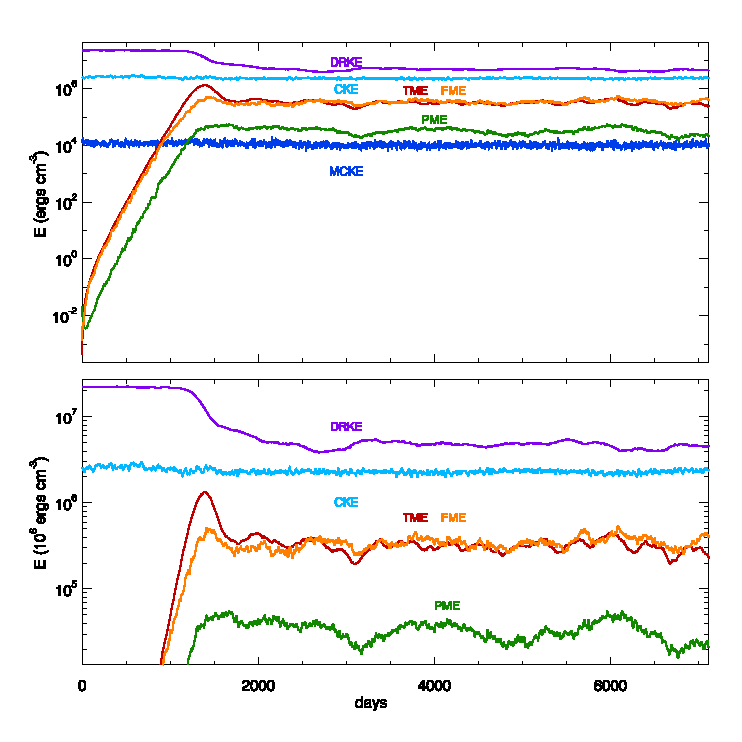
\includegraphics[width=0.85\linewidth]{figs/chapter_2/apj_energy_trace_mmc_vturf_3.eps}
  \end{center}
  \caption[Evolution of kinetic and magnetic energies in dynamo case~D3]
	  {Evolution of kinetic and magnetic energies in dynamo case~D3. 
	    $(a)$ Volume-averaged kinetic energy densities of differential
	  rotation (DRKE), convection (CKE) and meridional
	  circulations (MCKE) shown in logarithmic plot.  Magnetic
	  energy densities in fluctuating magnetic fields (FME), mean
	  toroidal fields (TME) and mean poloidal fields (PME) are
	  shown growing from an initial seed field.  The dynamo
	  saturates after roughly 1700~days.  After saturation, DRKE
	  has changed substantially but CKE and MCKE are largely unaffected.
	  $(b)$ Zoom in logarithmic plot of evolving kinetic and
	  magnetic energies, emphasizing their behavior after
	  saturation.
	  Time is counted from day~0, when the last adjustments were
	  made to parameters controlling the simulation
	  (i.e. $\Omega_0$, $\eta$, etc.).
  \label{fig:energy_D3}}
  %\vspace{0.5cm}
\end{figure}
%%%%%%%%%%%%%%%%%%%%%%%%%%%%%%%%%%%%%%%%%%%%%%%%%%%%%%%%%%%%%%%%%%%%%



These dynamo simulations are computationally intensive, requiring both
high spatial resolution to correctly represent the velocity fields and long
time evolution to capture the equilibrated dynamo behavior, which may
include cyclic variations on time scales of hundreds to thousands of days.  The strong
magnetic fields can produce rapidly moving Alfv\'en waves which
seriously restrict the Courant-Friedrichs-Lewy (CFL) timestep limits
in the upper portions of the convection zone.  Case~D3, rotating three
times faster than the current Sun, has been evolved for over 7000 days
(or over 2 million timesteps with typical timesteps of 300~seconds), and case~D5, rotating five times faster
than the Sun, has seen more than 17000 days of evolution (representing
more than 10 million timesteps, with typically 140~seconds of evolution per timestep).

These two cases were conducted at magnetic Prandtl number $\mathrm{Pm}
= \nu/\eta =0.5$, a value significantly lower than employed in our
previous solar simulations.  In particular, \cite{Brun_et_al_2004}
explored $\mathrm{Pm} =2,2.5$ and $4$, and \cite{Browning_et_al_2006}
studied $\mathrm{Pm}=8$.  The high magnetic Prandtl numbers were
required in the solar simulations to reach sufficiently high magnetic
Reynolds numbers to drive sustained dynamo action.  In the simulations
of \cite{Brun_et_al_2004} only the simulations with $\mathrm{Pm} >2.5$
and $\mathrm{Rm}' \gtrsim 300$ achieved sustained dynamo action, where
$\mathrm{Rm}'$ is the fluctuating magnetic Reynolds number.  We are
here able to use a lower magnetic Prandtl number for three reasons.
Firstly, more rapid rotation tends to stabilize convection and lower
values of $\nu$ and $\eta$ are required to drive the convection.  Once
convective motions begin however they become quite vigorous and the
fluctuating velocities saturate at values comparable to our solar
cases.  Thus the Reynolds numbers achieved are fairly large and we can
achieve modestly high magnetic Reynolds numbers even at low
$\mathrm{Pm}$.  Secondly, the differential rotation becomes
substantially stronger with both more rapid rotation $\Omega_0$ and
with lower diffusivities $\nu$ and $\eta$.  This global-scale flow is
an important ingredient and reservoir of energy for these dynamos, and
the increase in its amplitude means that low $\mathrm{Pm}$ dynamos can
still achieve large magnetic Reynolds numbers based on this zonal
flow.  Thirdly, the critical magnetic Reynolds number for dynamo action
likely decreases with increasing kinetic helicity
\citep[e.g.,][]{Leorat_et_al_1981}.  Helicity generally increases with
rotation rate \citep[e.g.,][]{Kapyla_et_al_2009}, so the rapidly
rotating flows considered here achieve dynamo action at somewhat lower
$\mathrm{Rm}$ than the models of \cite{Brun_et_al_2004}, which rotated
at the solar rate.



Case~D3, which builds persistent wreaths of magnetism, is presented in
Chapter~\ref{chapter:case D3}.  Case~D5 at five times the solar rate has
time-dependent wreaths that flip global-scale polarity and is
presented in Chapter~\ref{chapter:case D5}. 
An analysis of terms contributing to building and destroying the
persistent magnetic fields is carried out for case~D3 in
Chapter~\ref{chapter:dynamo production}.
A variety of other dynamo cases, some at higher turbulence levels and
rotation rates, will be in turn discussed in Chapter~\ref{chapter:menagerie of dynamos}.




